% Chapter 3

\chapter{Solution n° 2} % Main chapter title

\label{Chapter3} % For referencing the chapter elsewhere, use \ref{Chapter3}

%----------------------------------------------------------------------------------------
\begin{description}
  \item[Plateforme :] i.MX6
  \item[Version du Kernel :] 3.14
  \item[Source :] \href{https://chromium.googlesource.com/chromiumos/third_party/kernel/+/factory-ryu-6486.14.B-chromeos-3.14/drivers/media/i2c/soc_camera/imx219.c}
  {https://chromium.googlesource.com/chromiumos/third\_party/kernel/+/factory-ryu-6486.14.B-chromeos-3.14/drivers/media/i2c/soc\_camera/imx219.c} \\
\end{description}


\section{Fichiers sources}
Ce driver contient les fonctions de configuration de l’imx219 : on, off, gain,
couleurs, taille de l’affichage. Il repose sur les couches de driver i2c et v4l.
La configuration du périphérique imx219 effectuée par v4l-utils est automatique
lors du chargement du module. Elle s’appuie sur les trois couches de driver
imx219>v4l>i2c. Le flux vidéo configuré peut ensuite être récupéré par Gstreamer.

\section{Travail effectué}
\begin{itemize}
\item[-] Gstreamer permettrait de streamer le flux sur le réseau à travers le protocole
UDP alors que v4l-utils permettrait plutôt d’enregistrer le flux vidéo.
\item[-] Création d’une recette
\end{itemize}

%\section{L’arborescence des fichiers in-tree}
%\begin{figure}[th]
%    \centering
%    \decoRule
%    \caption{Arborescnce des fichiers}  \label{fig:arbor}
%end{figure}

\section{Compilation de driver}
Extrait de la recette : récupère le fichier imx219.c, le compile par la cross
tool-chain et l’installe

\begin{lstlisting}
SUMMARY = "driver imx219"
SECTION = "examples"
LICENSE = "MIT"
LIC_FILES_CHKSUM = "file://${COMMON_LICENSE_DIR}/MIT;md5=c2b5f7071fdde268bf46ace1546f3c4b"

SRC_URI = "file://imx219.c"

S = "${WORKDIR}"

do_compile() {
         ${CC} imx219.c -o imx219
}

do_install() {
         install -d ${D}${bindir}
         install -m 0755 imx219 ${D}${bindir}
}
\end{lstlisting}

\section{Utilisation du driver sur la cible}
Vérification de la présence du driver dans l’arborescence :

%\begin{figure}[th]
%    \centering
%    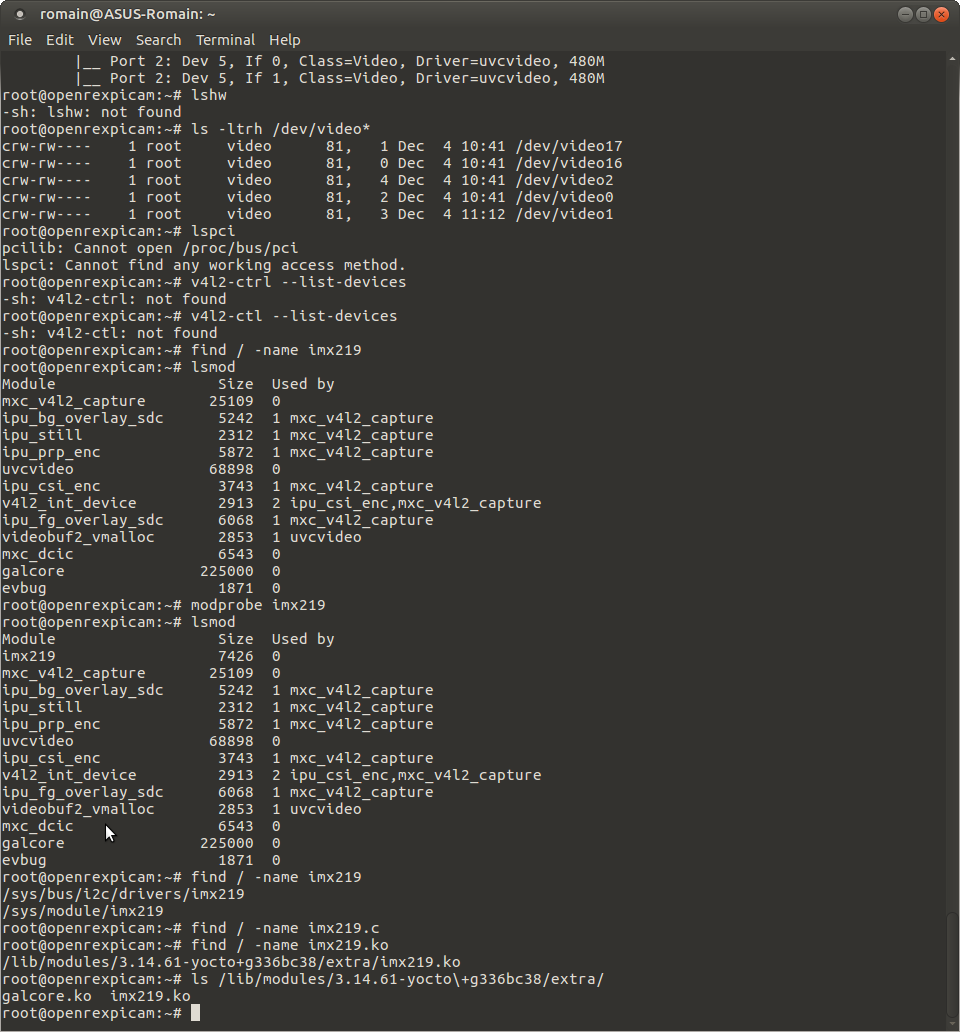
\includegraphics[width=1\linewidth,trim={0cm 1cm 0cm 33,1cm},clip]{presence.png}
%    \decoRule
%    \caption{Vérification de la présence du driver}  \label{fig:pres}
%\end{figure}

Chargement du module imx219 :

%\begin{figure}[th]
%    \centering
%    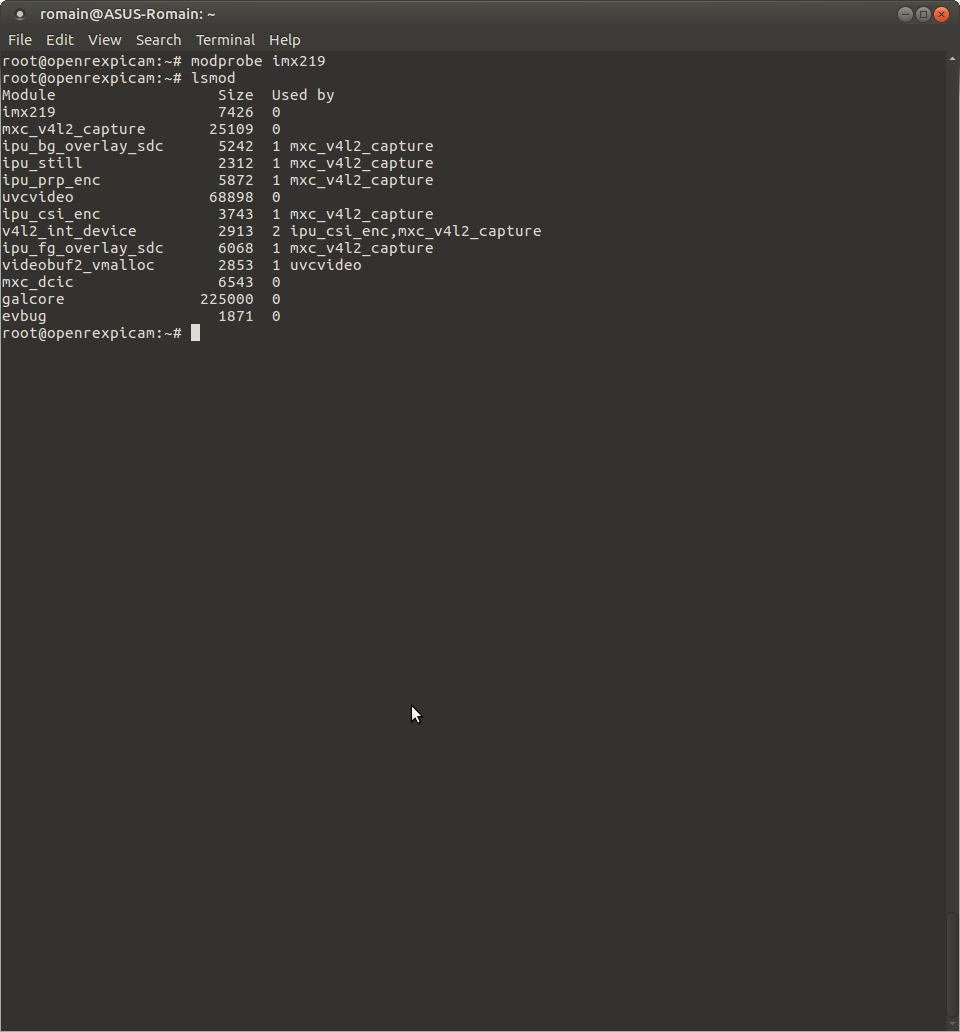
\includegraphics[width=1\linewidth,trim={0cm 25cm 0cm 1,8cm},clip]{module.png}
%    \decoRule
%    \caption{Chargement du module}  \label{fig:mod}
%\end{figure}

Comme nous pouvons le voir le driver n’est pas encore utilisé par v4l (Used by 0).

\clearpage

Chargement du module à l’adresse I2C de l’imx219 :

%\begin{figure}[th]
%    \centering
%    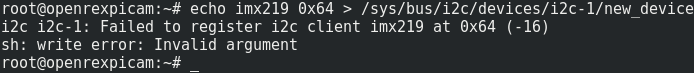
\includegraphics[width=1\linewidth]{modadd.png}
%    \decoRule
%    \caption{Chargement du module avec l'adresse I2C}  \label{fig:modadd}
%\end{figure}

Erreur sur le bus i2c sur laquelle nous travaillons actuellement.
Récupération du flux vidéo en local via Gstreamer :

\textbf{\# gst-launch-1.0 v4l2src device="/dev/videoX" ! video/x-raw,width=640,height=480 ! autovideosink}

X’ étant le numéro correspondant au numéro du driver vidéo du port CSI-2

Actuellement nous cherchons l’utilisation des commandes gst-launch-1.0 et des
fichiers de configurations v4l2src (cf. Chapitre \ref{Chapter5}).

\section{Conclusion}

Cette solution est notre piste la plus concrète. En effet la compilation a réussi,
nous cherchons à comprendre comment utiliser le driver à travers v4l. Une fois cette
tache effectuée nous travaillerons sur le portage des versions du kernel (3.14 $\rightarrow$ 4.1).

%----------------------------------------------------------------------------------------
